\documentclass[../poliXuniversity_hospital_(USP)_report.tex]{subfiles}

\begin{document}
\chapter{Objetivo}

\subsection{Robo Hospitalar / Hema-Bot}

Dar continuidade ao Projeto piloto da parceria HU X POLI, Robô Hospitalar, fazendo melhorias técnicas e estéticas ao modelo proposto e fabricado anteriomente. Isso seria feito através da Terceira Versão do Robo, apelidado de Hema-BOT, nome inspirado célula sanguínea responsável pelo transporte de oxgénio e gás carbônico no corpo humano.

\begin{figure}[h]
\centering
    \caption{Robo modelo Hospi\cite{hospi}}
    \centering % para centralizarmos a figura
    %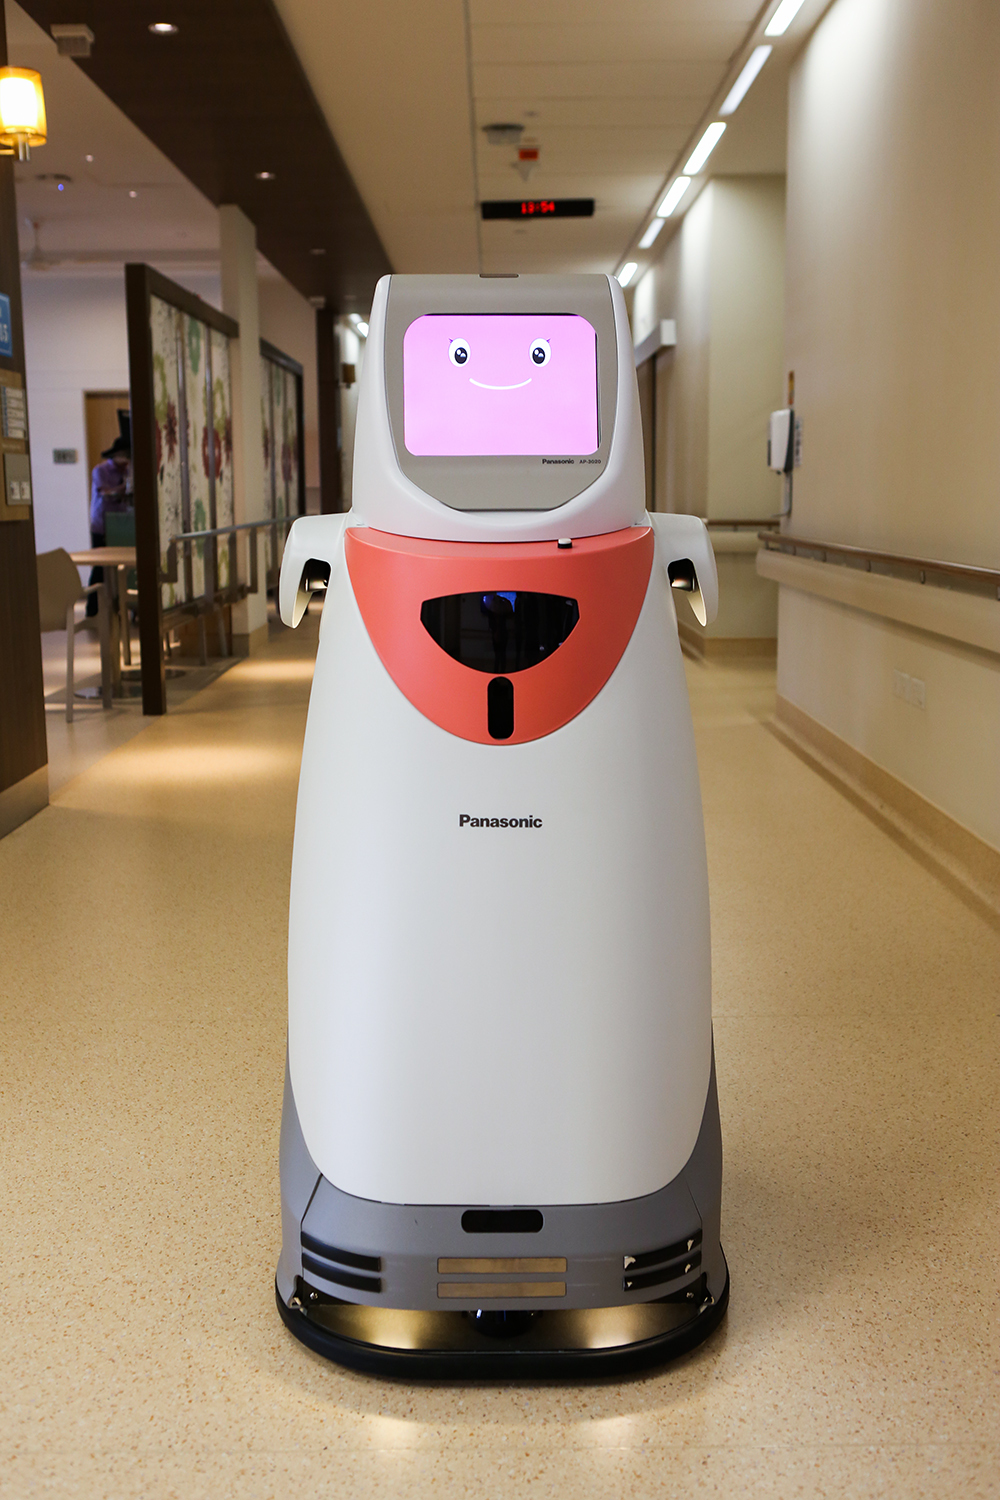
\includegraphics[width=11cm]{images/hospi.jpg}
    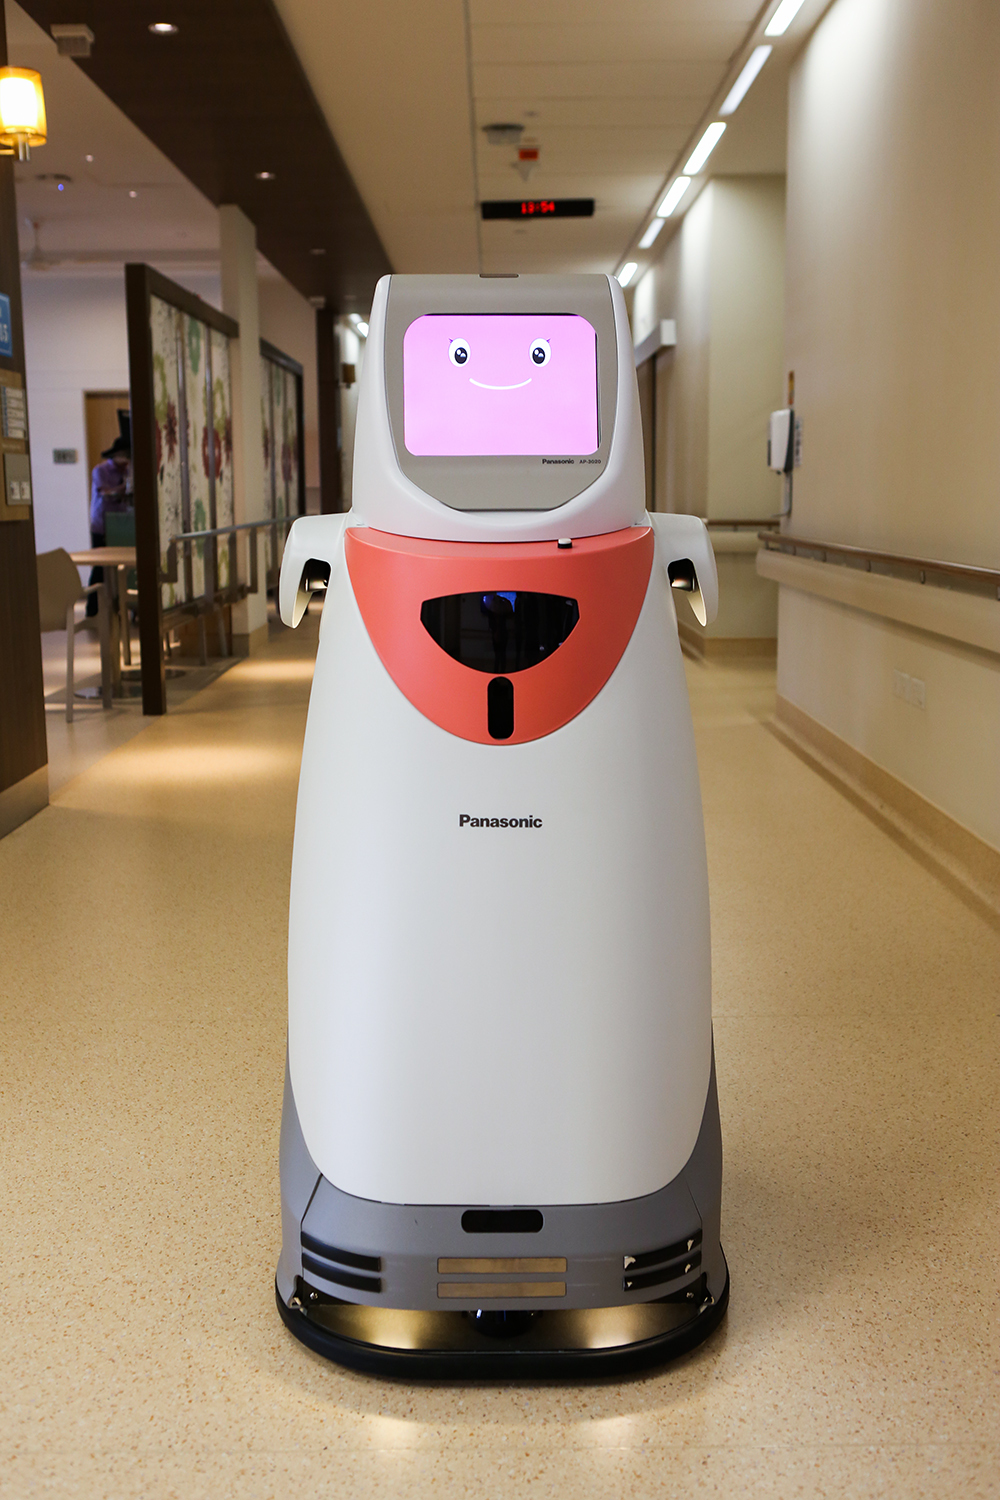
\includegraphics[width=7cm]{images/hospi.jpg}
    \caption*{Fonte: businesswire}
    \label{fig: Robô Hospi}
\end{figure}

\subsection{Ciclo Ergômetro}

Fazer a concepção e prototipação de um equipamento de reabilitação capaz de ser usado por paciente acamados com saúde debilitada. O equipamento deve auxiliar o movimento ou resisti-lo dependo da saúde do paciente, além disso o aparelho irá coletar dados como velocidade de rotação, quantidade de ciclos realizados e esforço médio. Em suma, será um ciclo ergometro com sistema de tração controlado(auxílio/resistência) que coleta e processa parâmetros importantes para mensurar a progressão do tratamento fisioteraoeutico do paciente.

\begin{figure}[h!]
\centering
    \caption{Aparelho(alemão) Reck Motomed\cite{reck}}
    \centering % para centralizarmos a figura
    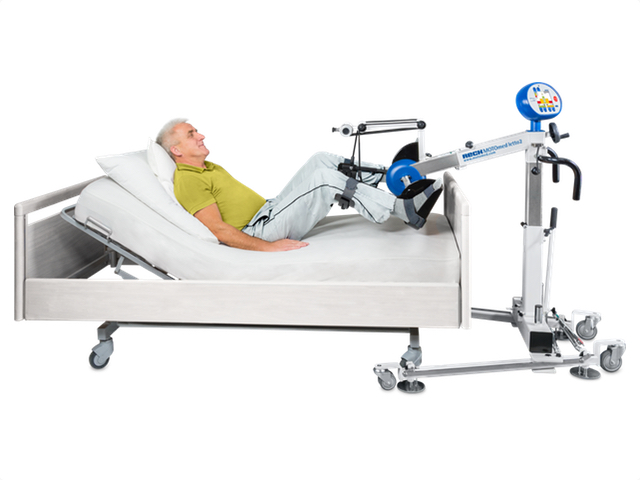
\includegraphics[width=11cm]{images/motomed.jpg}
    \caption*{Fonte: monteggia}
    \label{fig: Reck MOTOmed}
\end{figure}

\subsection{Automação da Farmácia / Golgi-Bot}

Realizar a concepção e fabricação de uma máquina selecionadora de remédios. Tal equipamento seria semelhante a uma vending-machine porém de remédios. Ela contaria com um sistema que permite realizar o controle de estoque farmaco, analise de estoque, registro de entrata e saida, autenticação via chave única e a programação de retirada automática dessas receitas. De maneria resumida, o equipamento faria a seleção dos remédios de maneria automática, manten-se assim registro de todas operações feitas pela máquina assim como os responsáveis por recarregar ou retirar medicamentos, o que garante a segurança do processo e a rastreabilidade de falhas na seleção, além do ganho de segurança a ela poderá operar 24 horas permitindo assim que a equipe da farmácia possa se dedicar integralmente ao cuidado do paciente.

\begin{figure}[ht]
\centering
    \caption{Maquina selecionadora modelo PillPick \cite{PillPick}}
    \centering % para centralizarmos a figura
    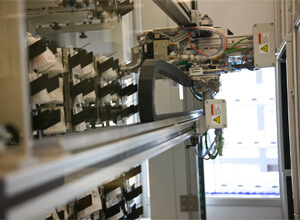
\includegraphics[width=11cm]{images/pillpick.jpg}
    \caption*{Fonte: monteggia}
    \label{fig: Pill Pick Swisslog}
\end{figure}

\end{document}